\documentclass[10pt, twocolumn]{article}
\usepackage[margin=1in]{geometry}
\usepackage{graphicx}
\usepackage{microtype}
\usepackage{nicefrac}
\usepackage{verbatim}
\usepackage{amsmath}
\usepackage{nicefrac}
\usepackage[colorlinks=false, hidelinks]{hyperref}
\usepackage{caption}
\usepackage{subcaption}
\usepackage{amsmath}
\usepackage{listings}
\usepackage{color}
\usepackage[dvipsnames]{xcolor}
\usepackage{tikz}
\usetikzlibrary{shapes, snakes, arrows, automata, positioning}

\definecolor{mygray}{rgb}{.9,.9,.9}
\lstset{ %
	breaklines=true
	language=[x86masm]Assembler,
  	backgroundcolor=\color{white},   % choose the background color; you must add \usepackage{color} or \usepackage{xcolor}
	numberstyle=\small\color{mygray}, % the style that is used for the line-numbers
	numbers=none,                    % where to put the line-numbers; possible values are (none, left, right)
}


\title{%
	\makebox[\textwidth][s]{%
		\hfill
		\begin{tabular}[b]{@{}c@{}}
				\fontsize{14}{20}\bfseries\selectfont \emph{Easy--PCB} Solder Reflow Oven\\
				\fontsize{12}{18}\selectfont Ben Lorenzetti\\
 		\end{tabular}%
    		\hfill
    		\makebox[0pt][r]{%
      			\includegraphics[width=0.2\textwidth]{Figures/easy-pcb-oven.pdf}}%
 	}% end makebox
}% end title

\author{}
\date{}

\begin{document}

\maketitle

\section*{Features}
\addcontentsline{toc}{section}{Features}

\begin{flushleft}
	\begin{itemize}
		\fontsize{10}{12}\bfseries\selectfont
		\item Insulated aluminum frame with XxYxZ interior chamber
		\item XXX Watt heating element with solid state relay control
		\item 120 VAC power supply with surge and short protection
		\item Forced convection fan driven by bipolar stepper motor with speed control
		\item Type X thermocouple for temperature feedback loop
		\item PIC18F14K50 based control
		\item Convenient \mbox{7--segment} display and pushbutton user interface
	\end{itemize}
\end{flushleft}

\section*{Introduction}
\addcontentsline{toc}{section}{Introduction}

\emph{Easy--PCB} is a small, desktop convection oven for DIY reflow soldering at home.

As integrated circuits continue to become smaller and faster,
many $\mu$Controllers, FPGAs, and other ICs are no longer available in
DIP form for breadboard prototyping or iron soldering.
Similar to the shift away from PC parallel ports in the early 2000s,
the shift away from DIPs means modern electronics hobbyists need more
complicated equipment than their predessesors.

Currently, commercial solder reflow stations are available for
soldering fine pitch, SMD, and BGA componenets.
More recently, several hackers have created open source designs
for inexpensive reflow ovens, using converted kitchen toaster ovens.

\emph{Easy--PCB} is better because it is a convection oven;
controlled air flow prevents parts from being blown out of position and
convection heating obviates the uneven heat absorbtion seen in infrared radiation based systems.
Furthermore, \emph{Easy--PCB} was designed from the ground up for soldering,
so the heating elements and oven frame were optimized alongside the
temperature controller for a typical solder reflow profile.

\begin{center}
	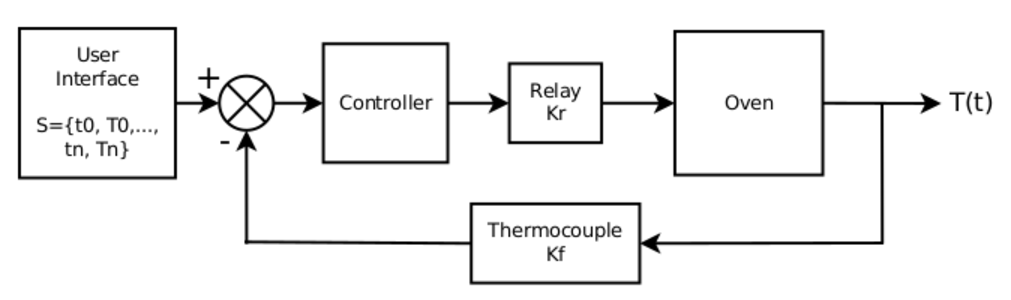
\includegraphics[width=\columnwidth]{Figures/control-system.pdf}
	\captionof*{figure}{The \emph{Easy--PCB} Control System: not just a controller bolted onto a disjoint oven.}
\end{center}

\emph{Easy--PCB} allows hobbyists to produce reflow temperature profiles with
a high degree of accuracy and repeatability.
Alongside freely available PCB design programs like Eagle and low-quantity
fabrication services like OSH Park, \emph{Easy--PCB} makes
modern integrated components, such as digital CMOS cameras,
within the design space of hobbyists and hackers.

\begin{center}
	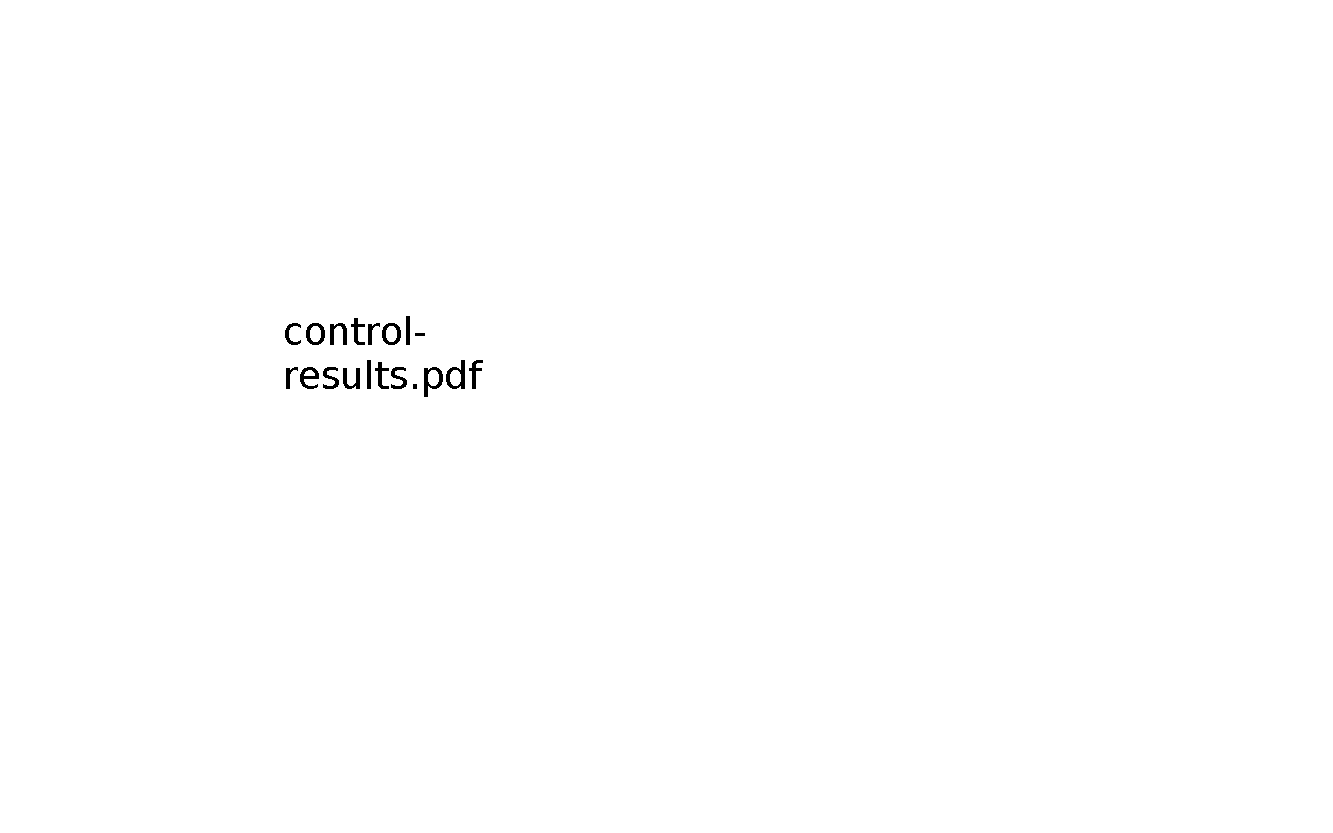
\includegraphics[width=\columnwidth]{Figures/control-results.pdf}
	\captionof*{figure}{Faithful Temperature Profile Control}
\end{center}

\tableofcontents

\section{User Interface}

\emph{Easy--PCB} presents temperature and time information on a four digit LED display.
After pressing the green `start' button, the current temperature and process
runtime are alternately displayed every second.

\begin{center}
	\begin{minipage}[b]{0.45\columnwidth}
		\centering
		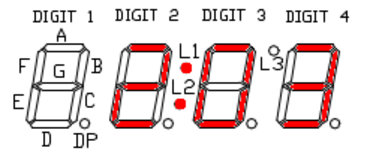
\includegraphics[width=\textwidth]{Figures/clock-display.pdf}
	\end{minipage}
	\begin{minipage}[b]{0.45\columnwidth}
		\centering
		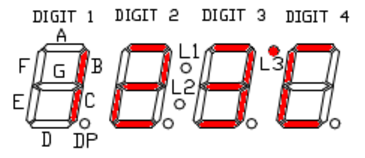
\includegraphics[width=\textwidth]{Figures/temperature-display.pdf}
	\end{minipage}	
%	\captionof*{figure}{Time and Temperature Displays}
\end{center}

The red `stop' button can be pressed at anytime to quit the current process
or reset the microcontroller.

\begin{center}
	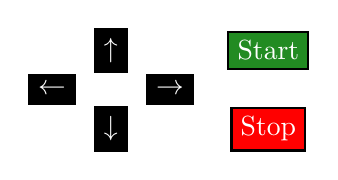
\begin{tikzpicture}[font=\fontsize{10pt}{11pt}\selectfont]
		\node [draw, thick,fill=black] (left) at (0cm, 0.5cm) {\textcolor{white}{$\leftarrow$}};
		\node [draw, thick,fill=black] (right) at (1.5cm, .5cm) {\textcolor{white}{$\rightarrow$}};
		\node [draw, thick, fill=black] (up) at (0.75cm, 1cm) {\textcolor{white}{$\uparrow$}};
		\node [draw, thick, fill=black] (down) at (0.75cm, 0cm) {\textcolor{white}{$\downarrow$}};
		\node [draw, thick, fill=ForestGreen] (start) at (2.75cm, 1cm) {\textcolor{white}{Start}};
		\node [draw, thick, fill=red] (stop) at (2.75cm, 0cm) {\textcolor{white}{Stop}};
	\end{tikzpicture}
	\captionof*{figure}{Pushbutton Interface}
\end{center}

Set point programming with the 4 nav keys is used to enter a time--temperature profile.
Use the `left' and `right' keys to move between set points and the `up' and `down'
keys to edit each set point value.

\begin{center}
	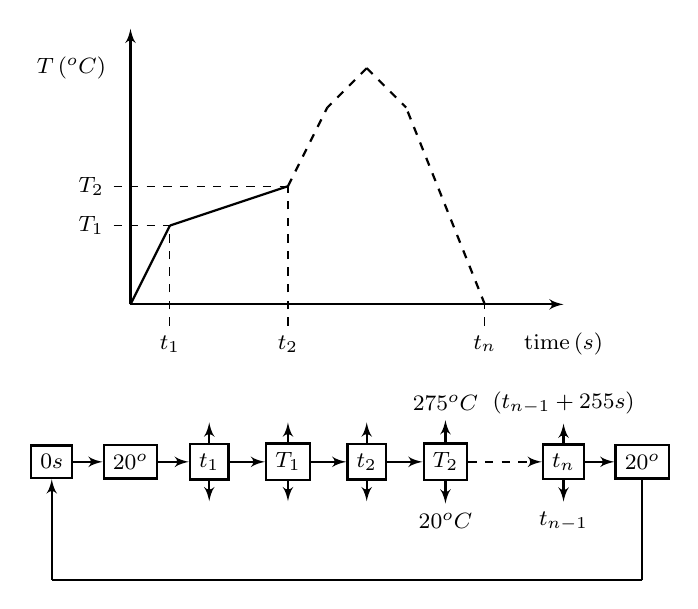
\begin{tikzpicture}[font=\fontsize{8pt}{9pt}\selectfont]
		\path [draw, -latex', thick] (1cm, 4cm) -- (1cm, 7.5cm);
		\path [draw, -latex', thick] (1cm, 4cm) -- (6.5cm, 4cm);
		\path [draw, thick] (1cm, 4cm) -- (1.5cm, 5cm);
		\path [draw, thick] (3cm, 5.5cm) -- (1.5cm, 5cm);
		\path [draw, thick, dashed] (3cm, 5.5cm) -- (3.5cm, 6.5cm);
		\path [draw, thick, dashed] (4cm,7cm) -- (3.5cm, 6.5cm);
		\path [draw, thick, dashed] (4cm,7cm) -- (4.5cm, 6.5cm);
		\path [draw, thick, dashed] (5.5cm,4cm) -- (4.5cm, 6.5cm);
		\node [draw, thick] (tzero) at (0cm, 2cm) {$0s$};
		\node [draw, thick] (Tzero) at (1cm, 2cm) {$20^{o}$};
		\path [draw, -latex', thick] (tzero) -- (Tzero);
		\node [draw, thick] (tone) at (2cm, 2cm) {$t_{1}$};
		\path [draw, -latex', thick] (Tzero) -- (tone);
		\node [draw, thick] (Tone) at (3cm, 2cm) {$T_{1}$};
		\path [draw, -latex', thick] (tone) -- (Tone);
		\node [draw, thick] (ttwo) at (4cm, 2cm) {$t_{2}$};
		\path [draw, -latex', thick] (Tone) -- (ttwo);
		\node [draw, thick] (Ttwo) at (5cm, 2cm) {$T_{2}$};
		\path [draw, -latex', thick] (ttwo) -- (Ttwo);
		\node [draw, thick] (tn) at (6.5cm, 2cm) {$t_{n}$};
		\path [draw, -latex', thick, dashed] (Ttwo) -- (tn);
		\node [draw, thick] (Tn) at (7.5cm, 2cm) {$20^{o}$};
		\path [draw, -latex', thick] (tn) to (Tn);
		\path [draw, thick] (Tn) -- (7.5cm, 0.5cm);
		\path [draw, thick] (7.5cm, 0.5cm) -- (0cm, 0.5cm);
		\path [draw, -latex', thick] (0cm,0.5cm) -- (tzero);
		\path [draw, -latex', thick] (tone) -- (2cm, 2.5cm);
		\path [draw, -latex', thick] (tone) -- (2cm, 1.5cm);
		\path [draw, -latex', thick] (Tone) -- (3cm, 2.5cm);
		\path [draw, -latex', thick] (Tone) -- (3cm, 1.5cm);
		\path [draw, -latex', thick] (ttwo) -- (4cm, 2.5cm);
		\path [draw, -latex', thick] (ttwo) -- (4cm, 1.5cm);
		\node (TtwoMax) at (5cm, 2.75cm) {$275^{o}C$};
		\node (TtwoMin) at (5cm, 1.25cm) {$20^{o}C$};
		\node (tnMax) at (6.5cm, 2.75cm) {$(t_{n-1}+255s)$};
		\node (tnMin) at (6.5cm, 1.25cm) {$t_{n-1}$};
		\path [draw, -latex', thick] (Ttwo) -- (TtwoMax);
		\path [draw, -latex', thick] (Ttwo) -- (TtwoMin);
		\path [draw, -latex', thick] (tn) -- (tnMax);
		\path [draw, -latex', thick] (tn) -- (tnMin);
		\node (t1label) at (1.5cm, 3.5cm) {$t_{1}$};
		\node (t2label) at (3cm, 3.5cm) {$t_{2}$};
		\node (tnlabel) at (5.5cm, 3.5cm) {$t_{n}$};
		\node (T1label) at (0.5cm, 5cm) {$T_{1}$};
		\node (T2label) at (0.5cm, 5.5cm) {$T_{2}$};
		\path [draw, dashed] (t1label) -- (1.5cm, 5cm);
		\path [draw, dashed] (t2label) -- (3cm, 5.5cm);
		\path [draw, dashed] (T1label) -- (1.5cm, 5cm);
		\path [draw, dashed] (T2label) -- (3cm, 5.5cm);
		\path [draw, dashed] (tnlabel) -- (5.5cm, 4cm);
		\node (Tlabel) at (0.25cm, 7cm) {$T\,(^{o}C)$};
		\node (tlabel) at (6.5cm, 3.5cm) {$\textrm{time}\,(s)$};
	\end{tikzpicture}
	\captionof*{figure}{Set Point Programming}
	\label{set-point-programming}
\end{center}

A total of 128 set points can be entered. The first set point is always $(0s,\,20^{o}C)$,
and the process will terminate at the next occurance of $20^{o}$ in a point.
Temperatures can take any value in the range \mbox{$20^{o}C<T<275^{o}C=527^{o}F$.}
The time between two points must be between \mbox{$0<=t<255$ seconds.}

\section{Plant Design}

\subsection{Temperature Objectives}

\begin{figure*}
	\centering
	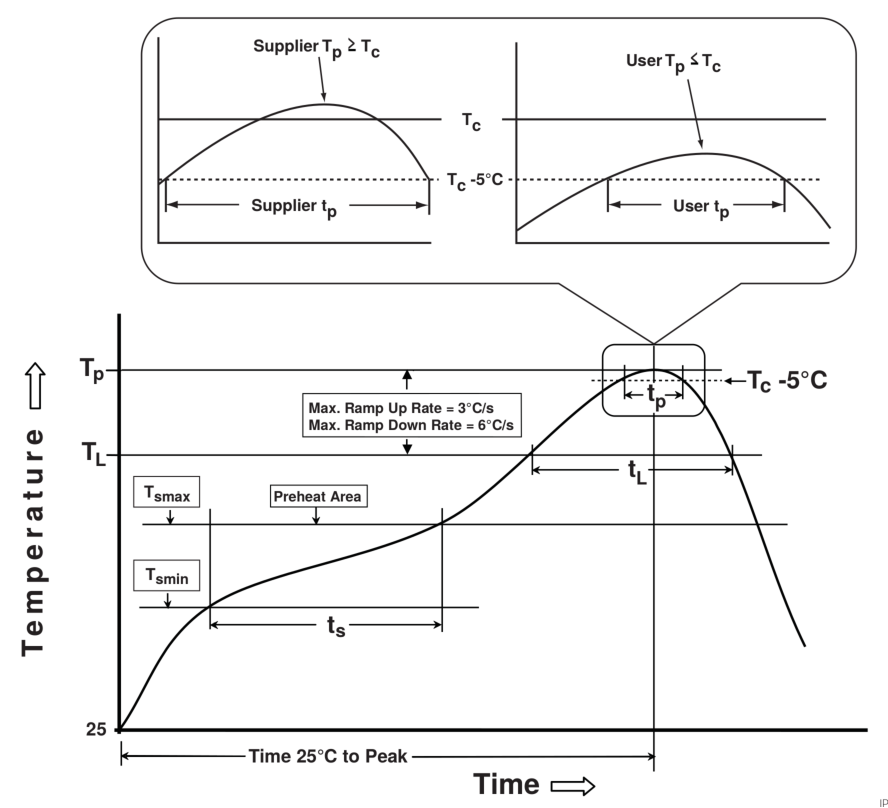
\includegraphics[width=0.7\textwidth]{Figures/standard-reflow-profile.pdf}
	\caption{Standard Solder Reflow Profile, per \href{J-STD-020D-1.pdf}{IPC/JEDEC STD-1-020D.1}}
	\label{standard-reflow-profile}
\end{figure*}

A typical solder reflow profile is shown in
\hyperref[standard-reflow-profile]{\mbox{figure \ref{standard-reflow-profile}}}.
The optimal shape and peak temperature depend on the components and,
more significantly, on the use of leaded solder.
\begin{equation*}
T_{p}\approx T_{c}=\left\{\begin{array}{c c}
220-235^{o}C	&\textrm{Leaded solder}	\\
245-260^{o}C	&\textrm{Pb--free}	\\
\end{array}\right.
\end{equation*}
\begin{equation*}
t_{p}=\left\{\begin{array}{c c}
20s	&\textrm{Leaded solder}	\\
30s	&\textrm{Pb--free}	\\
\end{array}\right.
\end{equation*}

\emph{Easy--PCB} was designed from the ground up for faithfully producing these
reflow profiles. This design process for the thermodynamic system is detailed below.

\subsection{Thermodynamics Theory}

\textbf{Heat} is everyone's least favorite form of energy because it
tends to dissipate everywhere and is difficult to transform into useful work.
Nevertheless, it is a form of energy so it is measured in joules.
\begin{equation*}
Q:=\textrm{Heat}\,[\textrm{Joules}]
\end{equation*}

From a microscopic view, heat is the kinetic energy of gas molecules or the
vibrational energy of bonds in solids. In both cases, summed over every
molecule, every bond, and every vibrational mode in the system.

\begin{center}
	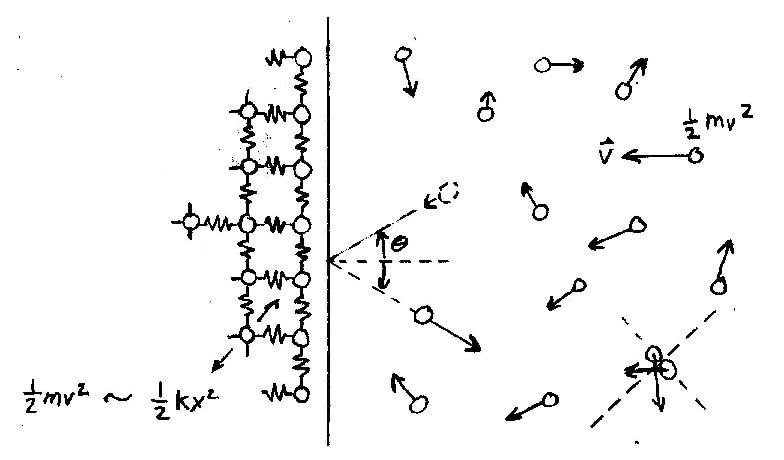
\includegraphics[width=1\columnwidth]{Figures/microscopic-view.pdf}
	\captionof{figure}{Heat Energy on a Molecular Scale}
	\label{microscopic-view}
\end{center}

\textbf{Temperature} is a potential field that measures an objects
tendancy to give up or absorb heat.
On average, heat always flows from regions of hotter temperature temperature
to lower temperature.
Temperature is usually measured in Kelvin or Celsius, which are related by
\begin{equation*}
T_{\textrm{Celsius}}=T_{\textrm{Kelvin}}+273.16.
\end{equation*}

Another way to think of temperature is a measure of heat density that also
incorporates the types of bonds (or lack thereof) in which heat energy is stored.
For example, a glacier contains more heat than a pot of boiling water, but
has a much lower heat density.

The relationship between temperature and heat stored in an object is given by
\begin{equation}
dQ=mc_{p}dT,
\label{specific-heat-eq}
\end{equation}
where $c_{p}$ is the specific heat of the material with units $\left[\frac{kJ}{kg*K}\right]$.

So heat flows spontaneously to reduce
temperature gradients, but how does heat flow and at what rate?
There are three mechanisms of heat transfer:
\emph{conduction}, \emph{convection}, and \emph{radiation}.

\textbf{Conduction} of heat is caused by molecular interactions,
such as the push--pull of nearby atomic bonds in solids or
elastic collisions between molecules of air.

The empirical relation for conduction is Fourier's Law, which
says the rate of heat transfer due to conduction is proportional
to both the difference in temperature and the media:
\begin{equation*}
\vec{q}=k\vec{\nabla}T
\end{equation*}
where $\vec{q}$ is the rate of heat transfer per unit surface area
and $k$ is the thermal conductivity of the medium with units
$\left[\frac{W}{m*K}\right]$.

In integral form, Fourier's Law is
\begin{equation*}
\frac{\delta Q}{\delta t}=k\oint_{S}\vec{\nabla}T*d\vec{A}.
\end{equation*}

And, in the one dimensional case,
\begin{equation}
\frac{\delta Q}{\delta t}=-kA\frac{\delta T}{\delta x}.
\label{1D-fouriers-law-eq}
\end{equation}

\textbf{Convection} is the second mechanism of heat transfer,
involving the bulk movement of particles driven by diffusion.

Every air molecule is moving in a random direction with random
kinetic energy, but a region of air with higher average kinetic
energy (temperature) will see more molecules leaving than entering
on average, because those leaving are moving faster than those
entering.

Note that in convection, no molecules gain or lose energy;
molecules of different energy simply trade places.

If a fan is used to apply work to a gas, the rate of convection
increases and then Newtons' Law of Cooling can predict the
rate of convection in gas near a solid surface of different
temperature.
\begin{equation}
\frac{dQ}{dt}=hA\Delta T
\label{newtons-cooling-law}
\end{equation}
where \(h\) is the heat transfer coefficient with \mbox{units \(\left[\frac{W}{m^{2}*K}\right]\)}.

\textbf{Radiation}, the third mechanism of heat transfer, is more
familiar to electrical engineers. In any material, electrons
have discrete amounts of energy based on the wave patterns that can
exist for the atomic geometry. When an electron spontaneously falls
to a less energetic patter, that energy is emitted as a photon of
light.

The classic, physics--history example is black body radiation,
when a metal is heated to high temperature and glows.
A more modern examle is the LED.

The empirical relation for radiation is the Stefan--Boltzmann Law,
which says that the total energy radiated, over all wavelengths
and per unit surface area, is proportional to the fourth power of
the body's temperature.
\begin{equation}
j^{*}=\sigma T^{4}
\end{equation}
where $\sigma$ is a proportionality constant derived from other
constants of nature.

\textbf{Mechanisms \& Media} Usually one mechanism of heat transfer
is dominant in a particular medium, so much so that we can ignore the
other two. Typically this means conduction in solids,
convection in fluids or gas, and radiation in space.
However, sometimes the picture is more complicated including
two cases in an oven:
\begin{enumerate}
	\item At the boundary of metal and air, where conduction
	and convection are both significant.
	\item In a thermocouple loop, where thermal diffusion (convection)
	of electrons is useful despite conduction still being dominant.
\end{enumerate}

\subsection{Thermodynamic Design}

Most microwaves draw between 600 and 1200 Watts of power.
An IR toaster oven may draw 1500 Watts into its lamps.
How much power does \emph{Easy-PCB} need to produce the required temperature profiles?

Our approach for answering this question is to browse available parts on McMaster.com,
imagine how they would be assembled into an oven,
and then model their thermodynamic response using SPICE.

A first conceptual design of \emph{Easy--PCB} is shown in
\hyperref[first-oven-concept]{figure \ref{first-oven-concept}}.

\begin{center}
	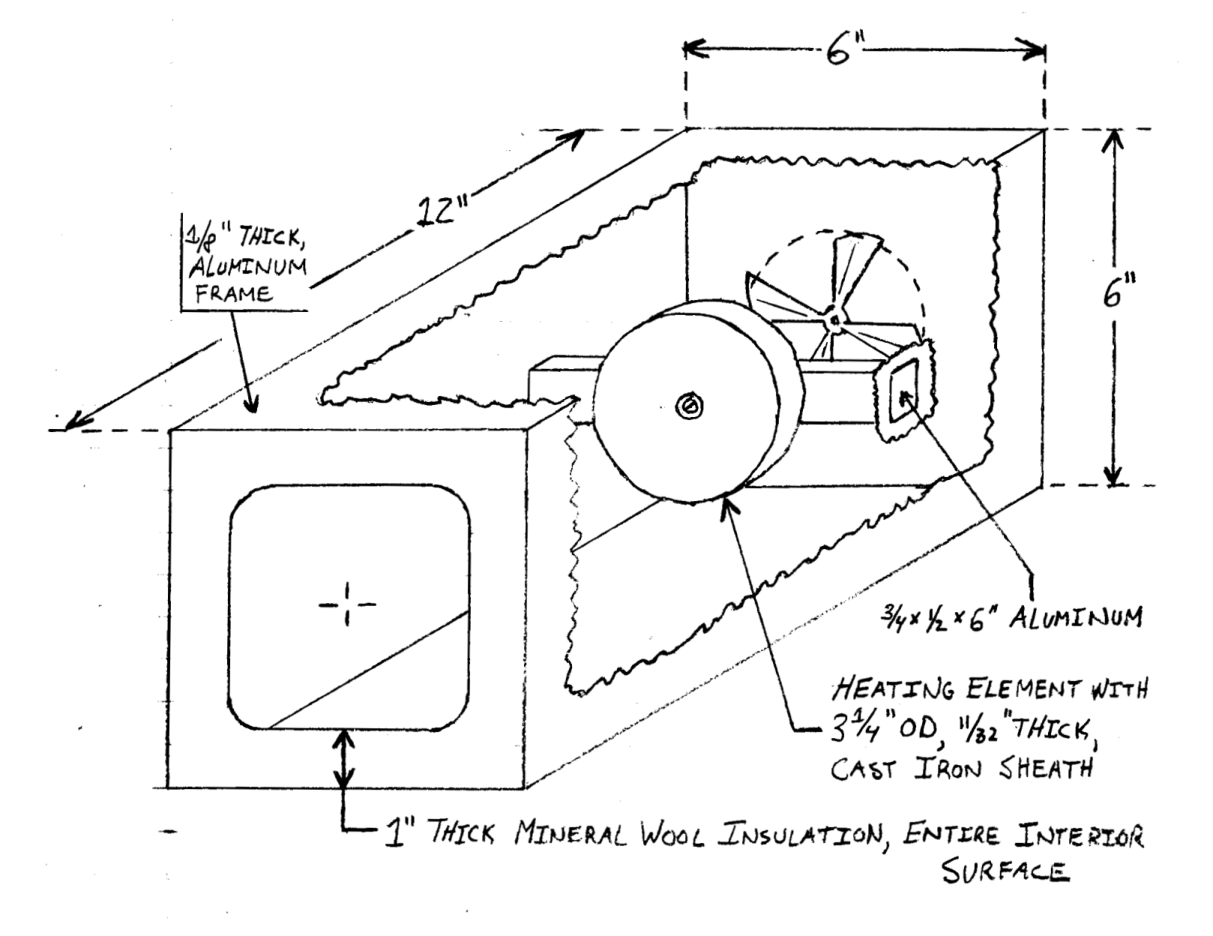
\includegraphics[width=\columnwidth]{Figures/first-oven-concept.pdf}
	\captionof{figure}{Concept for Thermodynamic System}
	\label{first-oven-concept}
\end{center}

\subsubsection*{Conduction through Metals \& Insulation}
In the concept, the oven chamber is isolated from the outside with walls of
mineral wool insulation and aluminum.
If the wall is relatively thin compared to the square root of its surface area,
then its heat transfer can be modeled as a 1--D transmission line, like shown in
\hyperref[unidirectional-conduction]{figure \ref{unidirectional-conduction}}.

\begin{center}
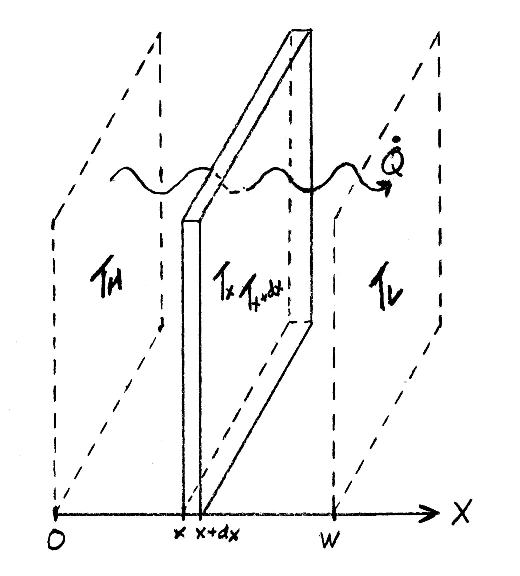
\includegraphics[width=0.85\columnwidth]{Figures/unidirectional-conduction.pdf}
\captionof{figure}{Heat Conduction in 1--D}
\label{unidirectional-conduction}
\end{center}

Assuming conduction is the dominant mechanism of heat transfer
and using Fourier's Law in 1--D,
(\hyperref[1D-fouriers-law-eq]{equation \ref{1D-fouriers-law-eq}})
the rate of heat passing through a thin slice is
\begin{equation*}
\frac{\delta Q}{\delta t}=-kA\frac{\delta T}{\delta x}
\end{equation*} 
 
And, from \hyperref[specific-heat-eq]{equation \ref{specific-heat-eq}},
the heat capacity of a thin slice of the metal sheath is
\begin{equation*}
dQ=(\rho A dx)c_{p}dT
\end{equation*}

Rewriting these equations to look like current-voltage relationships gives
\begin{equation}
\delta T=R_{x}\frac{\delta Q}{\delta t},
\quad R_{x}=\frac{\delta x}{kA}
\label{differential-resistance-eq}
\end{equation}
and
\begin{equation}
\frac{\delta Q}{\delta t}=C_{x}\frac{\delta T}{\delta t},
\quad C_{x}=\rho A c_{p} * \delta x
\label{differential-capacitance-eq}
\end{equation}

Values for thermal conductivity $k$, specific heat capacity $c_{p}$, and 
density $\rho$ of different materials are listed in
\hyperref[thermal-properties-table]{table \ref{thermal-properties-table}}.

Long metal bars and rods can also be modeled with equations
\ref{differential-resistance-eq} and \ref{differential-capacitance-eq}
if the heat loss along the length of the bar is assumed to be
negligible compared to heat transfered at the end faces.

\begin{center}
	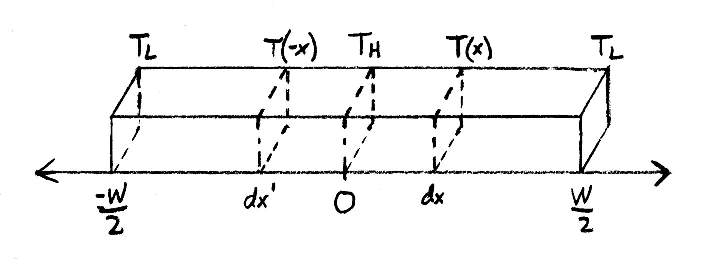
\includegraphics[width=1\columnwidth]{Figures/bidirectional-conduction.pdf}
	\captionof{figure}{1--D Conduction in Both Directions}
	\label{bidirectional-conduction}
\end{center}

For metal components where heat is injected at the center
of the part and dissipates symmetrically in either direction,
such as the support bar shown in
\hyperref[bidirectional-conduction]{figure \ref{bidirectional-conduction}}
or the metal sheath encasing the heating element,
the surface area can be doubled so that the transmission line
only needs to be integraded in the positive direction.
\begin{equation}
\left\{\begin{array}{c c c}
A_{x}	&\Rightarrow	&2A_{x}	\\
R_{x}	&\Rightarrow	&R_{x}/{2}	\\
C_{x}	&\Rightarrow	&2C_{x}	\\
\{x|-\frac{w}{2} \leq x \leq \frac{w}{2}\}	&\Rightarrow	&\{x|0 \leq x \leq \frac{w}{2}\}	\\
\end{array}\right.
\end{equation}

\begin{table*}
\centering
\caption{Thermal Conductivity, Specific Heat, and Density of Selected Materials}
\begin{tabular}{c | c | c | c | c}
\hline\hline
Material	&Linear Range $(^{o}C)$	&k \(\left(\frac{W}{m*K}\right)\)	&\(c_{p}\) \(\left(\frac{kJ}{kg*K}\right)\)	&\(\rho\) \((kg/m^{3})\)	\\
% Material	k	Cp	density	\\
\hline
Type 6061 Aluminum		&25	&167	&0.896	&2700	\\
Type 304 Stainless Steel	&0--100	&16.2	&0.5	&8000	\\
Cast Iron			&25	&55.0	&0.46	&6800--7800	\\
1.0 K--factor Insulation	&-	&0.1442	&-	&-	\\
0.23 K--factor Insulation	&-	&0.0332	&-	&-	\\
\hline\hline
\end{tabular}
\label{thermal-properties-table}
\end{table*}

\subsubsection*{Conductivity of Metal--Air Interface}

In the bulk volume of air, convection is the dominant form of heat
transfer and collisions are relatively rare. However, where the
air meets a solid surface, the net convection must go to zero because
there can be no net movement of air molecules into the solid.
Furthermore, every air molecule that reaches the surface experiences
a collision so there is 100\% conduction at the surface.

For some distance away from the surface, there is a larger than
normal chance of head--on collisions and slower rates of diffusion
due to the nearby wall. In this region, both conduction and convection
may be significant. To analyze this transition region,
we will start at the surface where there is 100\% conduction
because that is the mechanism we have equations for.

From the first law of thermodynamics, the rate of heat being stored
in a differential volume is equal to the rate of heat entering less
the rate of heat leaving the volume element.
\begin{equation*}
\frac{\delta Q_{\textrm{stored}}}{\delta t}=
\frac{\delta Q_{\textrm{in}}}{\delta t}-
\frac{\delta Q_{\textrm{out}}}{\delta t}
\end{equation*}

Looking back at
\hyperref[unidirectional-conduction]{figure \ref{unidirectional-conduction}},
the differential volume element is a plane, so
\begin{equation*}
\frac{\delta Q_{\textrm{stored}}}{\delta t}=
\frac{\delta Q_{x}}{\delta t}-
\frac{\delta Q_{x+\delta x}}{\delta t}.
\end{equation*}

Substituting in
\hyperref[heat-capacity-eq]{equation \ref{specific-heat-eq}}
for stored heat capacity and
\hyperref[1D-fouriers-law-eq]{equation \ref{1D-fouriers-law-eq}} for
conduction through the element yields a transport equation.

\begin{equation}
mc_{p}\frac{\delta T}{\delta t}=kA\frac{\delta T}{\delta x}
\label{transport-eq}
\end{equation}

This cannot be solved analytically unless space and time are independent.
Sorry Albert.
\begin{equation}
T(x\,,t)=T_{x}(x)*T_{t}(t)
\end{equation}

Applying the chain rule to equation \ref{transport-eq}
\begin{equation*}
mc_{p}\frac{\delta T_{t}(t)}{\delta t}T_{x}(x)=
kA\frac{\delta T_{x}(x)}{\delta x}T_{t}(t)
\end{equation*}
and separating variables gives
\begin{equation*}
mc_{p}\frac{\delta T_{t}(t)}{\delta t}*\frac{1}{T_{t}(t)}=
kA\frac{\delta T_{x}(x)}{\delta x}*\frac{1}{T_{x}(x)}.
\end{equation*}

The only way for the equality to be true for all space and time
is if both sides are equal to a common constant.
\begin{equation*}
\alpha=mc_{p}\frac{\delta T_{t}(t)}{\delta t}*\frac{1}{T_{t}(t)}
\end{equation*}
\begin{equation*}
\alpha=kA\frac{\delta T_{x}(x)}{\delta x}*\frac{1}{T_{x}(x)}
\end{equation*}

Each of these can be solved by separation of variables.
\begin{equation*}
\frac{\alpha}{kA}\delta x=\frac{\delta T_{x}(x)}{T_{x}(x)}
\end{equation*}

\begin{equation*}
\frac{\alpha}{kA}\int \delta x=\int \frac{1}{T_{x}(x)}*\delta T_{x}(x)
\end{equation*}

\begin{equation*}
\frac{\alpha x}{kA}=ln\left(T_{x}(x)\right)+\beta_{1}
\end{equation*}

\begin{equation*}
T_{x}(x)=\beta_{1}^{'}e^{\nicefrac{\alpha x}{kA}}
\end{equation*}

Similarly for time,
\begin{equation*}
T_{t}(t)=\beta_{2}^{'}e^{\nicefrac{\alpha t}{mc_{p}}}.
\end{equation*}

Recombining the independent components gives
\begin{equation*}
\Delta T(x\,,t)=\beta_{1}^{'}\beta_{2}^{'}e^{\nicefrac{\alpha x}{kA}+\nicefrac{\alpha t}{mc_{p}}}
\end{equation*}

The boundary conditions are that at $t=0$ and $x=0$, the temperature difference is
the initial temperature difference, and at $t\rightarrow\infty$ and $x\rightarrow\infty$,
the temperature difference dissipates to zero.
\begin{equation*}
\Delta T(x\,,t)=\Delta T_{0}e^{\nicefrac{-\alpha x}{kA}-\nicefrac{\alpha t}{mc_{p}}}
\end{equation*}

Now, for the sake of physical intuition we can write
\begin{equation}
\Delta T(x\,,t)=\Delta T_{0}e^{-(\nicefrac{x}{\delta}+\nicefrac{t}{\tau})},
\label{transport-solution-eq}
\end{equation}
where $\delta$ is a `skin depth' over which the spacial gradient decays to $1/e$ its
initial value and $\tau$ is a time constant related to the skin depth by
\begin{equation}
\tau=\frac{mc_{p}}{kA}\delta.
\label{transport-time-constant-eq}
\end{equation}

Make some arguments and plot the temperature and heat transfer curves.
Assume steady state and somehow that active cooling makes it all valid.

Applying Fourier's law to the temperature profile found in
\hyperref[transport-solution-eq]{equation \ref{transport-solution-eq}},
gives us the rate of heat trasfer in the air due to conduction.
\begin{equation*}
\frac{dQ}{dt}=-kA\frac{dT}{dx}=
\frac{kA}{\delta}\Delta T_{0}e^{-(\nicefrac{x}{\delta}+\nicefrac{t}{\tau})}
\end{equation*}

Again assuming steady state, the rate of heat trasfer at any distance from
the wall is equal to the rate of conduction at the wall.
\begin{equation}
\frac{dQ}{dt}=\frac{kA}{\delta}\Delta T_{0}=h_{c}A\Delta T_{0}
\label{derived-cooling-law-eq}
\end{equation}

This is the information we were after and, ironically, it turns out this is 
Newton's Law of Cooling
(\hyperref[newtons-cooling-law]{equation \ref{newtons-cooling-law}})
where $h_{c}=\nicefrac{k}{\delta}$. Since we do not have any way of predicting
the skin depth except by experimentation, some common values for
the convective heat transfer coefficient $h_{c}$ are listed in
\hyperref[typical-h-values-table]{table \ref{typical-h-values-table}}.

\begin{table}
	\centering
	\caption{Typical Convective Heat Transfer Coefficients}
	\begin{tabular}{c | c | c}
	\hline\hline
	Fluid	&Conv.	&$h_{c}\,\left[\frac{W}{m^{2}*K}\right]$	\\
	\hline
	Gases, \& dry vapors	&free	&$0.5-1000$	\\
				&forced	&$10-1000$	\\
	Water \& liquids	&free	&$50-3000$	\\
				&forced	&$50-10000$	\\
	Boiling Water		&-	&$3-100$	\\
	Condensing $H_{2}O$ Vapor&-	&$5-100$	\\
	\hline\hline
	\end{tabular}
	\label{typical-h-values-table}
\end{table}

\hyperref[derived-cooling-law-eq]{Equation \ref{derived-cooling-law-eq}}
can be rewrittent to look like Ohms' law for SPICE analysis.
\begin{equation}
\Delta T=R_{c}\frac{dQ}{dt},\quad R_{c}=\frac{1}{h_{c}A}=\frac{\delta}{kA}
\label{cooling-resistance-eq}
\end{equation}

\subsubsection*{Heat Capacity of Chamber Air}

The heat capacity of the air in the chamber cannot be analyzed
with constant coefficient assumptions.
\begin{equation}
dQ=m(T)c_{p}(T)dT
\label{specific-heat-with-variable-coefficients-eq}
\end{equation}

\begin{table}
	\centering
	\caption{Thermal Properties of Air}
	\begin{tabular}{c | c | c | c}
\hline\hline
$T\,[^{o}C]$	&$\rho\left[\frac{kg}{m^{3}}\right]$	&$c_{p}\left[\frac{kJ}{kg*K}\right]$	&$k\left[\frac{W}{m*K}\right]$	\\
\hline
20	&1.205	&1.005	&0.0257	\\
40	&1.127	&1.005	&0.0271	\\
60	&1.067	&1.009	&0.0285	\\
80	&1.000	&1.009	&0.0299	\\
100	&0.946	&1.009	&0.0314	\\
120	&0.898	&1.013	&0.0328	\\
140	&0.854	&1.013	&0.0343	\\
160	&0.815	&1.017	&0.0358	\\
180	&0.779	&1.022	&0.0372	\\
200	&0.746	&1.026	&0.0386	\\
250	&0.675	&1.034	&0.0421	\\
300	&0.616	&1.047	&0.0454	\\
\hline\hline
	\end{tabular}
	\label{air-properties-table}
\end{table}

From \hyperref[air-properties-table]{table \ref{air-properties-table}},
we can see that the specific heat of air does not vary much over the
temperature range of the oven; less than 0.3\% from $c_{p(20^{o}C)}$
over the range $20-300^{o}C$. However, the density and mass of air
in the chamber may change significantly.

Assuming that the air in the chamber behaves like an ideal gas
and is made up of the normal percentages of $N_{2}$, $O_{2}$, $CO_{2}$, etc., then mass and temperature are related by
\begin{equation*}
PV=\frac{m}{M}RT\quad\Rightarrow\quad m(T)=\frac{MPV}{R}T
\end{equation*}
where the ideal gas constant is
\begin{equation*}
R=5.00745\,\left[\frac{\textrm{atm}*\textrm{in}^{3}}{\textrm{mol}*K}\right]
\end{equation*}
and the molar mass of air is
\begin{equation*}
M=28.97\,\left[\frac{g}{\textrm{mol}}\right]
\end{equation*}

For the first oven concept in
\hyperref[first-oven-concept]{figure \ref{first-oven-concept}},
the volume of the chamber is fixed in natural units of $in^{3}$
and there are likely small leaks that let the chamber
pressure equilibrate to atmospheric pressure $1\,\textrm{atm}$.

Substituting $m(T)$ into
\hyperref[specific-heat-with-variable-coefficients-eq]
{equation \ref{specific-heat-with-variable-coefficients-eq}},
converting from absolute Kelvin scale to Celsius, and
manipulating to look like a current--voltage relationship results in
\begin{equation}
\frac{dQ}{dt}=C_{c}(T)\frac{dT}{dt}
\end{equation}
where
\begin{equation}
C_{c}(T)=\frac{c_{p(20^{o}C)}MPV}{R}*\left(T+273.16^{o}C\right).
\end{equation}

Equivalently,
\begin{equation*}
C_{c}(T)=\left(5.8143\left[\frac{J}{in^{3}}\right]\right)V*(T+273.16^{o}C).
\end{equation*}


\subsection{Component Selection \& SPICE Modeling}

\subsection{Transfer Model}

\section{Thermocouple Amplifier Design}

\subsection{Controller and Power Requirements}

\section{Motor Driver Design}

\subsection{Power Requirements}

\section{Power Circuit Design}

\section{Controller Design}

\end{document}
